\chapter[Planejamento]{Planejamento}
\label{cap:planejamento}

Antes de iniciar o desenvolvimento do projeto, foi feita uma pesquisa sobre as regras do jogo de xadrez.
Em seguida, foram especificados os recursos necessários para a montagem do sistema e sua utilização.
Esta seção descreve as regras do jogo, a escolha do equipamento e o projeto inicial do sistema.

\section[Regras de xadrez]{Regras de xadrez}
\label{sec:xadrezRegras}

O jogo de xadrez é um jogo de tabuleiro para dois jogadores.
Sua origem é incerta, mas acredita-se que ele tenha surgido na Índia, antes mesmo da era cristã \cite{xadrez_historia}.

\subsection[Tabuleiro]{Tabuleiro}
\label{sub:xadrezTabuleiro}

O tabuleiro de xadrez é composto por 64 casas quadradas, alternadamente claras e escuras, dispostas em uma grade 8x8 conforme a Figura \ref{fig:xadrezTabuleiro}.
Cada casa é identificada por uma letra de \textit{a} a \textit{h} e um número de \textit{1} a \textit{8}
e pode comportar no máximo uma peça.

\begin{figure}[H]
    \centering
    \caption{Tabuleiro de xadrez}
    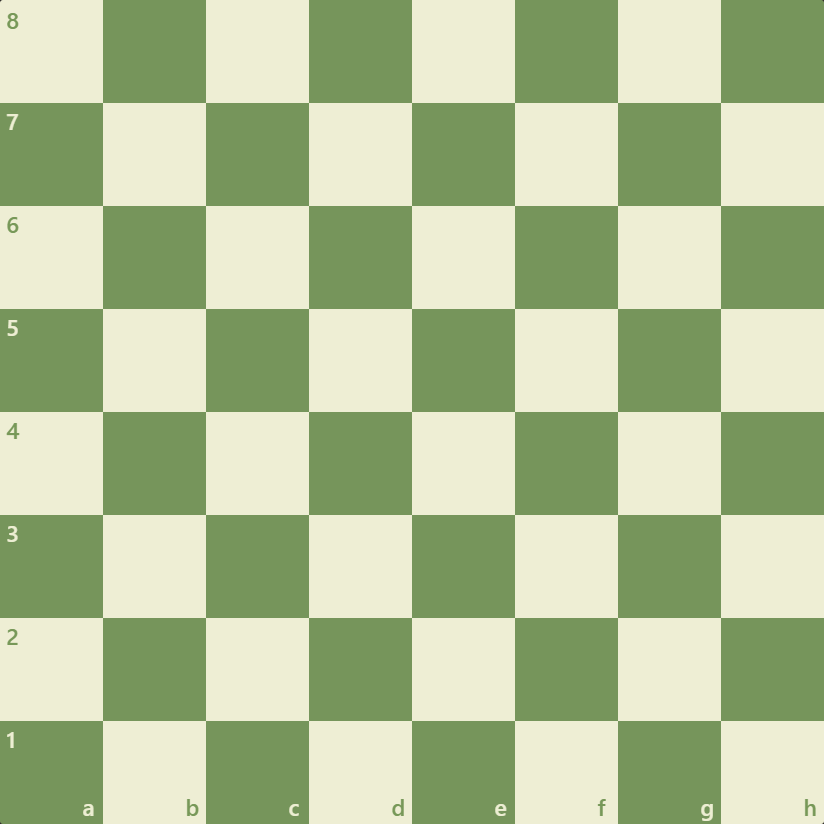
\includegraphics[keepaspectratio=true, width=0.6\textwidth]
    	{img/xadrez-tabuleiro.png}
    \fonte{\url{https://www.chess.com}}
    \label{fig:xadrezTabuleiro}
\end{figure}

\subsection[Peças]{Peças}
\label{sub:xadrezPecas}

O jogo de xadrez possui 6 tipos de peças ilustradas na Figura \ref{fig:xadrezPecas}.
Cada uma dessas peças utiliza diferentes regras para se movimentar pelo tabuleiro.

\begin{figure}[H]
    \centering
    \caption{Peças de xadrez}
    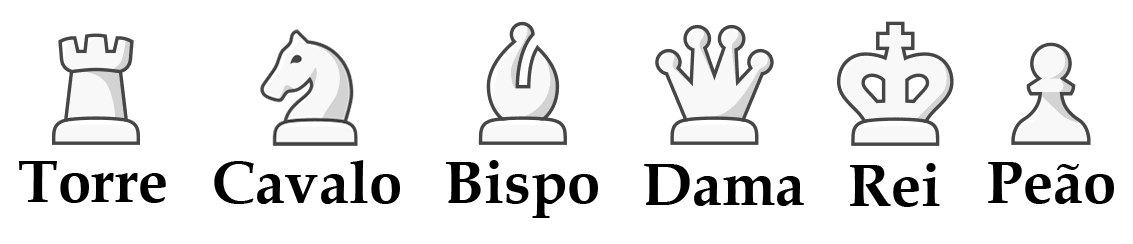
\includegraphics[keepaspectratio=true, width=0.6\textwidth]
    	{img/xadrez-pecas.png}
    \fonte{Do próprio autor}
    \label{fig:xadrezPecas}
\end{figure}

O Rei é a peça mais importante do jogo, e pode se mover para qualquer casa adjacente, horizontal, vertical ou diagonalmente.
Entretanto, ele não pode se mover para uma casa em que esteja em xeque, ou seja, em que ele possa ser capturado na próxima jogada.

A Torre pode se mover para qualquer casa na mesma linha ou coluna em que se encontra.
Por outro lado, o Bispo pode se mover para qualquer casa na mesma diagonal em que se encontra.

A Dama é a peça mais poderosa do jogo, e pode se mover como um Bispo ou como uma Torre,
ou seja, ela pode se deslocar para qualquer casa na mesma linha, coluna ou diagonal em que se encontra.

O Cavalo pode se mover duas casas em uma direção e uma casa em uma direção perpendicular, em forma de um \textit{L}.
Ele também é a única peça que pode pular outras peças.

Por fim, o Peão pode se mover uma casa para frente, ou duas casas para frente se ainda não tiver se movido no jogo.
Ele também pode capturar uma peça adversária que esteja uma casa na diagonal à sua frente.

\subsection[Início do jogo]{Início do jogo}
\label{sub:xadrezInicioJogo}

Para se iniciar uma partida de xadrez, o tabuleiro deve ser posicionado de forma que a casa \textit{a1} seja branca.
As peças brancas devem ser posicionadas na primeira linha,
seguindo a ordem: Torre, Cavalo, Bispo, Dama, Rei, Bispo, Cavalo e Torre.
As peças pretas devem ser posicionadas na oitava linha, seguindo a mesma ordem.
Os peões brancos devem ser posicionados na segunda linha e os peões pretos na sétima linha.
A Figura \ref{fig:xadrezTabuleiroMontado} apresenta o tabuleiro no início de uma partida.

\begin{figure}[H]
    \centering
    \caption{Tabuleiro de xadrez no início de uma partida}
    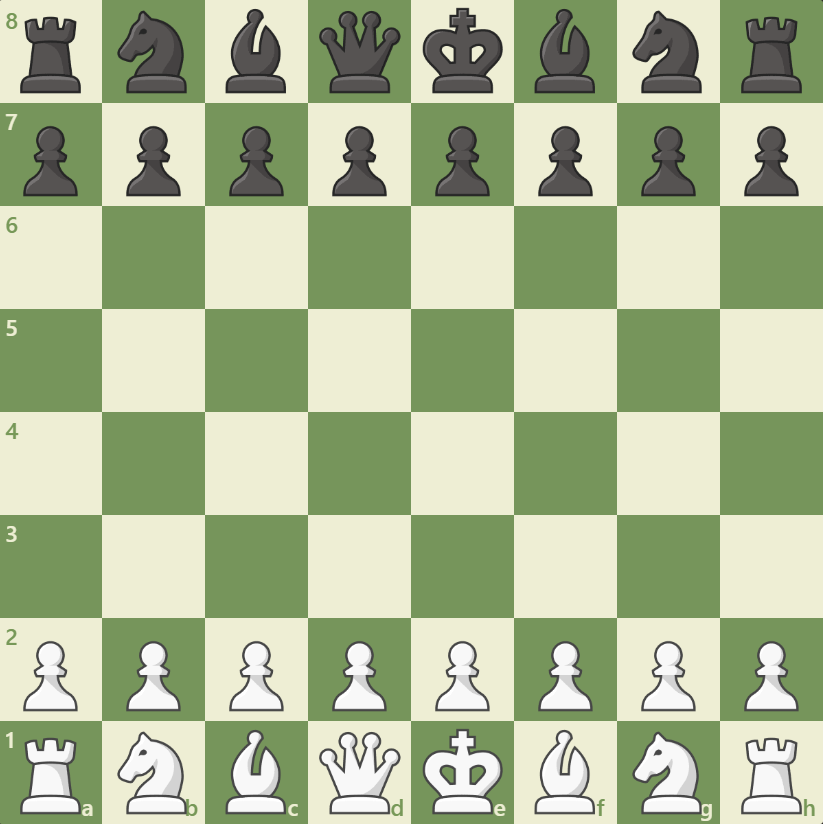
\includegraphics[keepaspectratio=true, width=0.6\textwidth]
    	{img/xadrez-tabuleiro-montado.png}
    \fonte{\url{https://www.chess.com}}
    \label{fig:xadrezTabuleiroMontado}
\end{figure}

Depois de montado o tabuleiro, o jogador que estiver com as peças brancas deve realizar a primeira jogada.
Em seguida, os jogadores devem realizar jogadas alternadas, até que o jogo termine conforme descrito na Subseção \ref{sub:xadrezFimJogo}.

\subsection[Fim de Jogo]{Fim de Jogo}
\label{sub:xadrezFimJogo}

O objetivo do jogo de xadrez é dar xeque-mate no Rei adversário, ou seja, deixar o Rei adversário em xeque e sem nenhuma casa para onde se mover.
Quando isso acontece, o jogo termina e o jogador que deu xeque-mate vence a partida.

Além disso, o jogo também pode terminar empatado.
Isso pode acontecer quando algum dos jogadores não possui nenhum movimento válido,
quando os jogadores concordam com o empate, quando o mesmo movimento é repetido três vezes
ou quando nenhum jogador tiver peças suficientes para dar xeque-mate.

\subsection[Movimentos especiais]{Movimentos especiais}

Além dos movimentos descritos na Subseção \ref{sub:xadrezPecas}, o jogo de xadrez possui alguns movimentos especiais.

O movimento de \textit{Roque} pode ser realizado pelo Rei e por uma Torre,
desde que ambas as peças ainda não tenham se movido no jogo e não haja nenhuma peça entre elas.
Para realizar o movimento, o Rei deve se mover duas casas em direção à Torre, e a Torre deve ser posicionada na casa adjacente ao Rei.
O movimento de \textit{Roque} pode ser realizado para a direita ou para a esquerda,
denominados \textit{Roque} curto e \textit{Roque} longo, com base na quantidade de casas que a Torre se move.

O movimento de \textit{En Passant} pode ser realizado por um Peão para capturar um Peão adversário em uma situação especial.
Caso o Peão adversário tenha se movido duas casas na jogada anterior, e esteja na mesma linha que um Peão capturador, é possível realizar o movimento de \textit{En Passant}.
Nesse caso, o Peão capturador deve se mover para a casa em que o Peão adversário estaria se tivesse se movido apenas uma casa na jogada anterior,
conforme ilustrado na Figura \ref{fig:xadrezEnPassant}.

\begin{figure}[H]
    \centering
    \caption{Movimento de \textit{En Passant}}
    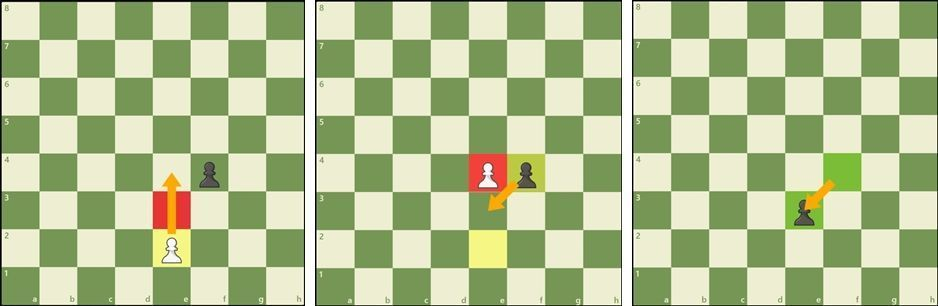
\includegraphics[keepaspectratio=true, width=0.9\textwidth]
    	{img/xadrez-enpassant.jpeg}
    \fonte{\url{https://www.chess.com}}
    \label{fig:xadrezEnPassant}
\end{figure}

O movimento de \textit{Promoção} pode ser realizado por um Peão quando ele chega na última linha do tabuleiro.
Nesse caso, o Peão deve ser substituído por uma Dama, Torre, Bispo ou Cavalo, conforme a escolha do jogador.
Não é permitido realizar o movimento de \textit{Promoção} para um Rei ou outro Peão.

\subsection[Notação]{Notação}
\label{sub:xadrezNotacao}

Para descrever os movimentos realizados em uma partida de xadrez, é utilizada a notação algébrica.
Nessa notação, é utilizada a identificação da casa do tabuleiro, conforme descrito na Subseção \ref{sub:xadrezTabuleiro},
e a identificação da peça que se moveu, conforme descrito na Tabela \ref{tab:xadrezNotacao}.

\begin{table}[H]
    \centering
    \caption{Notação das peças}
    \label{tab:xadrezNotacao}
    \begin{tabular}{|c|c|}
        \hline
        \textbf{Peça} & \textbf{Notação} \\ \hline
        Rei           & K               \\ \hline
        Dama          & Q               \\ \hline
        Torre         & R               \\ \hline
        Bispo         & B               \\ \hline
        Cavalo        & N               \\ \hline
        Peão          & -               \\ \hline
    \end{tabular}
\end{table}

Caso mais de uma peça possa realizar o mesmo movimento, é utilizada a notação da coluna em que a peça se encontra.
Além disso, é utilizada as notações \textit{O-O} e \textit{O-O-O} para representar os movimentos de \textit{Roque} curto e \textit{Roque} longo, respectivamente.
O símbolo \textit{x} é utilizado para representar uma captura.
Os símbolos \textit{+} e \textit{\#} são utilizados para representar um xeque e um xeque-mate, respectivamente.
Por fim, podem ser adicionados os símbolos \textit{!} e \textit{?} para representar um bom e um mau movimento, respectivamente.

A Tabela \ref{tab:xadrezNotacaoExemplo} apresenta alguns exemplos de notação algébrica.

\begin{table}[H]
    \centering
    \caption{Exemplos de notação algébrica}
    \label{tab:xadrezNotacaoExemplo}
    \begin{tabular}{|c|l|}
        \hline
        \textbf{Lançe} & \textbf{Descrição} \\ \hline
        e4             & Peão para a casa \textit{e4} \\ \hline
        exd5           & Peão da coluna \textit{e} captura a peça na casa \textit{d5} \\ \hline
        Qd8            & Dama para a casa \textit{d8} \\ \hline
        Qxd8           & Dama captura a peça na casa \textit{d8} \\ \hline
        Nf3!           & Cavalo para a casa \textit{f3} (movimento bom) \\ \hline
        Red1           & Torre da coluna \textit{e} para a casa \textit{d1} \\ \hline
        O-O?           & \textit{Roque} curto (movimento mau) \\ \hline
        Qe2+           & Dama para a casa \textit{e2} e xeque \\ \hline
        Qe2\#          & Dama para a casa \textit{e2} e xeque-mate \\ \hline
    \end{tabular}
\end{table}

\section[Escolha do equipamento]{Escolha do equipamento}
\label{sec:escolhaEquipamento}

Para o desenvolvimento do projeto, foram disponibilizados, pela instituição CEFET-MG, dois manipuladores robóticos e diversos dispositivos que podem ser utilizados para seu controle.
A partir desse equipamento, e de outros disponíveis no mercado, foi decidido como o projeto seria realizado.
Os equipamentos utilizados para o projeto estão descritos a seguir.

\subsection[Manipuladores]{Manipuladores}

Os principais elementos deste trabalho são os manipuladores robóticos, portanto foi feito inicialmente um estudo sobre seu funcionamento e sobre como seu controle pode ser realizado para movimentar as peças de xadrez.

Foi disponibilizado um manipulador robótico de modelo Mentor de cor preta, conforme a Figura \ref{fig:fotoManipuladorMentor}, e um manipulador de modelo RD5NT de cor azul, conforme a Figura \ref{fig:fotoManipuladorRD5NT}.
Eles possuem diversas juntas movimentadas por motores de corrente contínua, e permitem que o manipulador funcione de forma similar a um braço humano.
Além disso, cada junta possui um potenciômetro que indica a posição atual do eixo, por meio de um sinal analógico.

O manipulador Mentor apresenta 5 graus de liberdade e uma garra que pode ser utilizada para pegar e soltar objetos.
Além disso, ele possui caixas de redução em seus motores, o que permite que ele mantenha sua posição mesmo após o desligamento dos motores.
Suas dimensões e faixas de movimento são apresentadas na Tabela \ref{tab:caracteristicasManipuladorMentor} \cite{mentor_forward_kinematics}.

Já o manipulador RD5NT possui apenas 4 graus de liberdade e uma garra.
Além de não possuir caixa de redução em seus motores, ele utiliza molas em alguns eixos, o que faz com que perca sua posição quando os motores são desligados.
Portanto, seu controle deve ser realizado de forma contínua para que permaneça na posição desejada.
Suas dimensões e faixas de movimento são apresentadas na Tabela \ref{tab:caracteristicasManipuladorRD5NT} \cite{controle_neural_robo}.

\begin{table}
    \centering
    \caption{Características do manipulador robótico Mentor}
    \label{tab:caracteristicasManipuladorMentor}
    \begin{tabular}{|c|c|c|}
        \hline
        \textbf{Eixo} & \textbf{Movimento angular (graus)} & \textbf{Comprimento (mm)} \\ \hline
        Torso                    & 210 & 185 \\ \hline
        Ombro                    & 180 & 165 \\ \hline
        Cotovelo                 & 230 & 150 \\ \hline
        Esquerdo do Pulso        & 320 & 0   \\ \hline
        Direito do Pulso         & 320 & 0   \\ \hline
        Pulso \textit{Pitch} (Arfagem)    & 140 & -   \\ \hline
        Pulso \textit{Roll} (Rolamento)    & 320 & -   \\ \hline
    \end{tabular}
\end{table}

\begin{table}
    \centering
    \caption{Características do manipulador robótico RD5NT}
    \label{tab:caracteristicasManipuladorRD5NT}
    \begin{tabular}{|c|c|c|}
        \hline
        \textbf{Eixo} & \textbf{Movimento angular (graus)} & \textbf{Comprimento (mm)} \\ \hline
        Torso            & 293 & 110 \\ \hline
        Ombro            & 107 & 120 \\ \hline
        Cotovelo         & 284 & 160 \\ \hline
        Pulso            & 360 & 0   \\ \hline
    \end{tabular}
\end{table}

\begin{figure}[H]
    \begin{minipage}{.5\textwidth}
        \centering
        \caption{Manipulador robótico Mentor}
        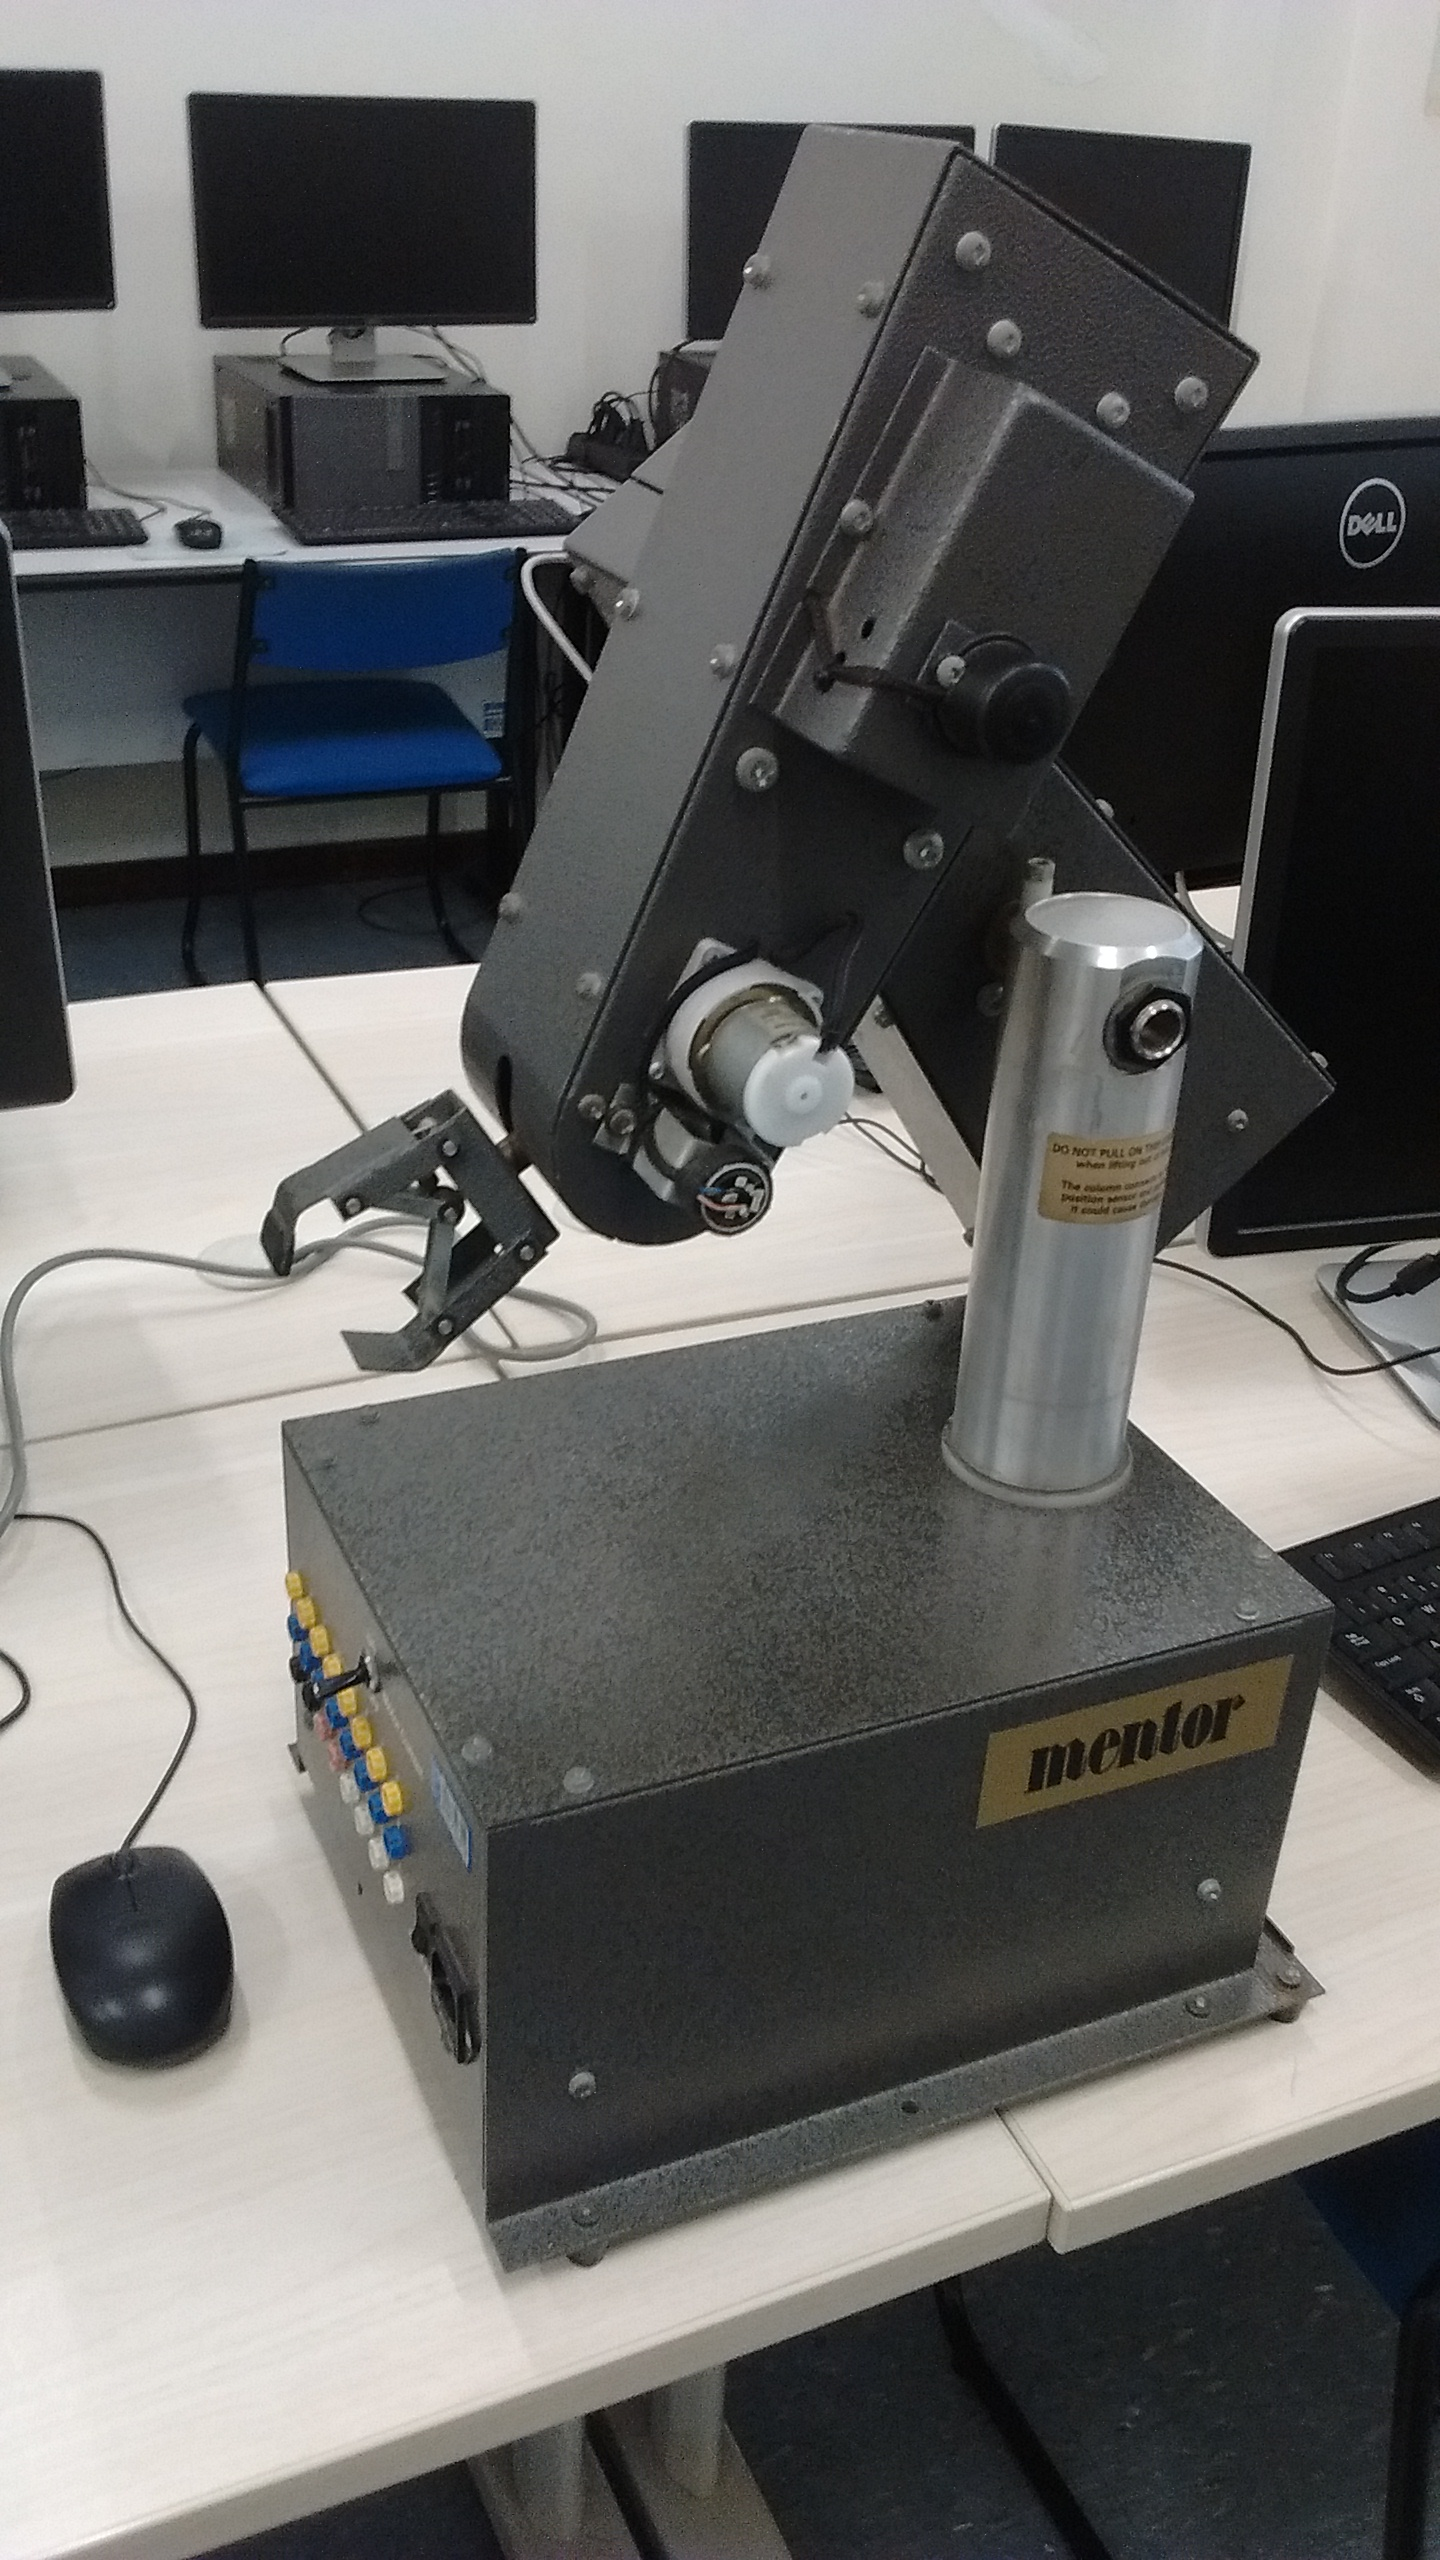
\includegraphics[keepaspectratio=true, width=0.9\linewidth]
            {img/foto-manipulador-preto.jpg}
        \fonte{http://arquivo.eng.br/robotica}
        \label{fig:fotoManipuladorMentor}
    \end{minipage}
    \begin{minipage}{.5\textwidth}
        \centering
        \caption{Manipulador robótico RD5NT}
        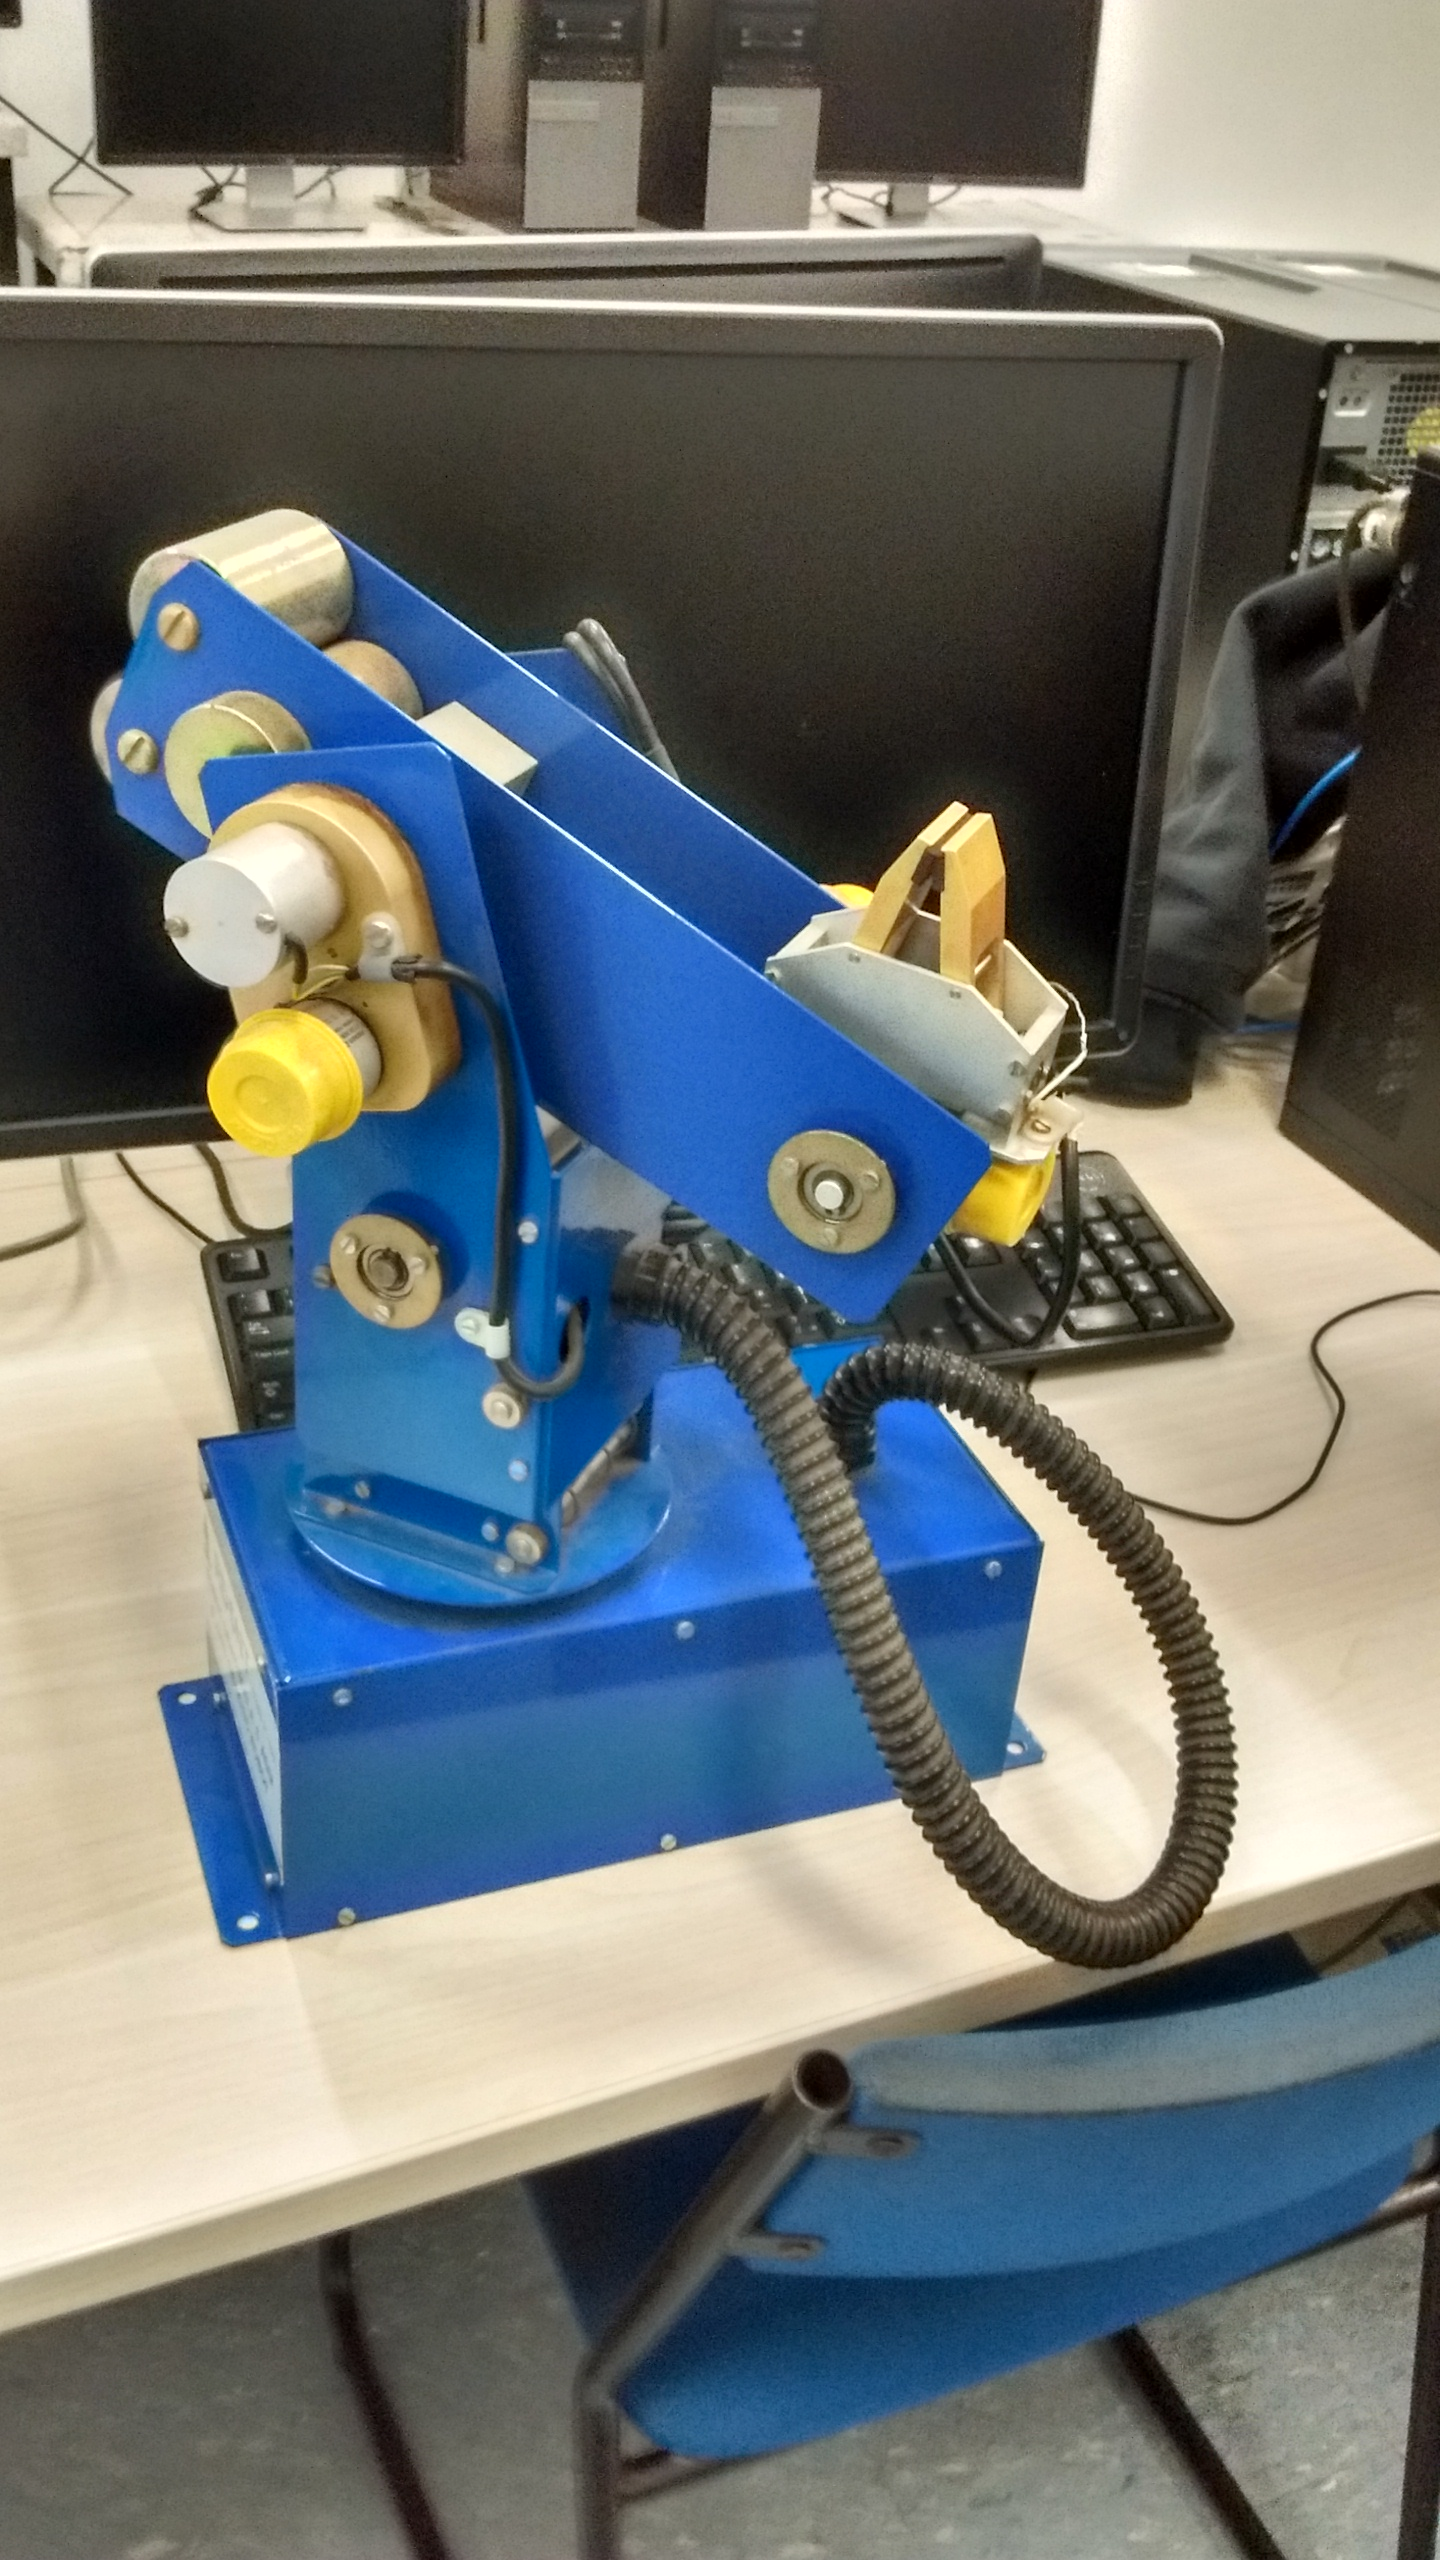
\includegraphics[keepaspectratio=true, width=0.9\linewidth]
            {img/foto-manipulador-RD5NT.jpg}
        \fonte{http://arquivo.eng.br/robotica}
        \label{fig:fotoManipuladorRD5NT}
    \end{minipage}%
\end{figure}

Foi decidido utilizar o manipulador de modelo RD5NT para o projeto, pois ele possui menos graus de liberdade na sua garra, o que facilita a implementação do algoritmo de controle.
Além disso, ele possui uma garra de tamanho adequado para pegar as peças de xadrez sem derrubar as outras peças do tabuleiro.
Apesar de não possuir caixa de redução em seus motores, isso não é um problema, pois o controle do manipulador será realizado de forma contínua.
A Figura \ref{fig:fotoBracoTabuleiro} apresenta o manipulador RD5NT ao lado de um tabuleiro de xadrez.

\begin{figure}[H]
    \centering
    \caption{Braço Robótico RD5NT ao lado de um tabuleiro de xadrez}
    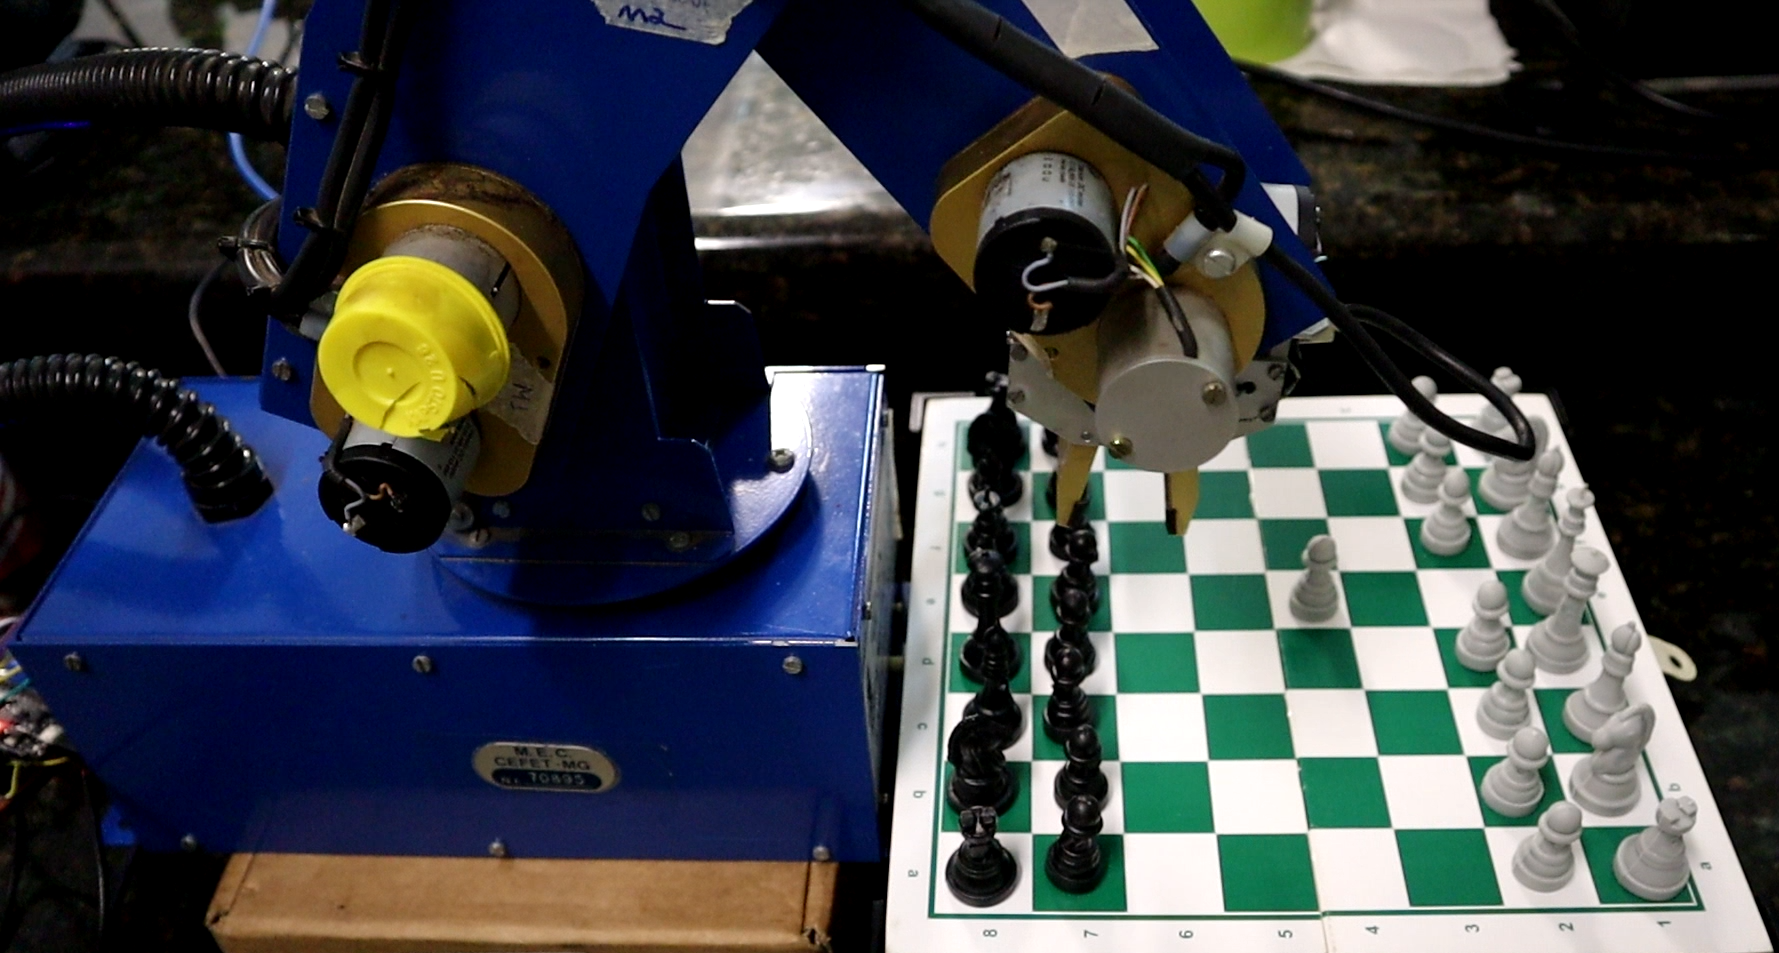
\includegraphics[keepaspectratio=true, width=0.9\textwidth]
    	{img/braco-tabuleiro.png}
    \fonte{Do próprio autor}
    \label{fig:fotoBracoTabuleiro}
\end{figure}

\subsection[Manete para o jogador]{Manete para o jogador}
\label{sub:maneteJogador}

Para que o jogador possa interagir com o manipulador, foi decidido utilizar uma manete de modelo \textit{batpad}, que possui dois \textit{joysticks}, conforme a Figura \ref{fig:fotoManeteJogador}.

Esses \textit{joysticks} devem ser alimentados com 3,3 ou 5 V e permitem a leitura de posição em duas dimensões, através de sinais analógicos.
Eles também possuem um botão que envia um sinal digital ao ser pressionado.

\begin{figure}[H]
    \centering
    \caption{Manete para o jogador}
    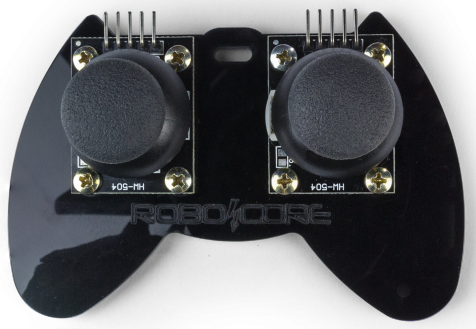
\includegraphics[keepaspectratio=true, width=0.5\textwidth]
    	{img/foto-controle-jogadores.png}
    \fonte{https://www.robocore.net/acessorios-robocore/controle-batpad}
    \label{fig:fotoManeteJogador}
\end{figure}

\subsection[Microcontrolador]{Microcontrolador}
\label{sub:microcontrolador}

Para realizar a integração entre a manete e o manipulador, foi decidido utilizar um microcontrolador ESP32, conforme a Figura \ref{fig:fotoESP32}.
Esse microcontrolador possui um \textit{clock} de 240MHz, 4MB de memória \textit{flash} e 320KB de memória \textit{RAM}.
Ele apresenta ao todo 34 pinos que podem ser utilizados como entrada ou saída, e suporta sinais analógicos e digitais \cite{esp32_datasheet}.

Para permitir o controle manual do manipulador robótico, o microcontrolador faz a leitura dos sinais analógicos e digitais provenientes da manete com alguns de seus 18 canais de \textit{ADC} (\textit{Analog to Digital Converter})[Conversor Analógico Digital].
E para permitir o controle automático, ele recebe sinais de controle de um computador através de um cabo USB.
A partir desses sinais, o ESP32 realiza o cálculo das posições desejadas de cada junta do manipulador.

Para controlar os motores, o microcontrolador primeiramente faz a leitura dos sinais analógicos provenientes dos potenciômetros de cada junta.
A partir desses sinais, é possível determinar a posição atual de cada junta.
Com base na posição atual e na posição desejada, o microcontrolador envia um sinal de controle para os motores do manipulador robótico, 
conforme apresentado na Figura \ref{fig:diagramaControle}.

\begin{figure}[H]
    \centering
    \caption{Diagrama de controle do sistema}
    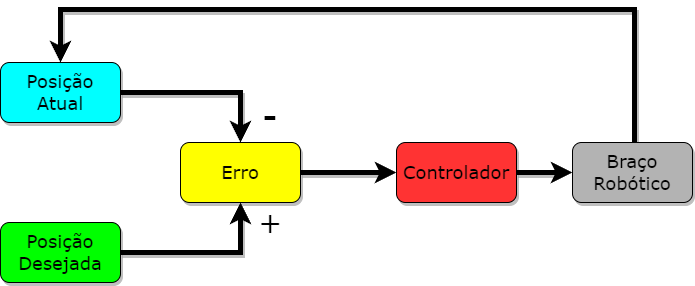
\includegraphics[keepaspectratio=true, width=0.9\textwidth]
    	{img/Diagrama Controle.png}
    \fonte{Do próprio autor}
    \label{fig:diagramaControle}
\end{figure}

Os sinais de controle são digitais do tipo \textit{PWM} (\textit{Pulse Width Modulation}), que variam de 0 a 3,3 V e possibilitam o controle da velocidade de rotação dos motores através da variação da tensão média.
Essa variação é feita através da escolha de valores diferentes de \textit{Duty Cycle} [Ciclo de Trabalho], que podem variar de 0\% a 100\%, e determinam a largura de pulso do sinal, conforme ilustrado na Figura \ref{fig:pwm}.
Valores maiores de \textit{Duty Cycle} resultam em maior velocidade de rotação do motor, pois o sinal permanece em nível alto por um período maior de tempo.
Por outro lado, valores menores de \textit{Duty Cycle} resultam em menor velocidade de rotação do motor, pois o sinal permanece em nível alto por um período menor de tempo.
Para definir o sentido de rotação do motor, foi utilizado um sinal digital que indica se ele deve girar no sentido horário ou anti-horário.

\begin{figure}[H]
    \begin{minipage}{.5\textwidth}
        \centering
        \caption{Largura do pulso do sinal de controle}
        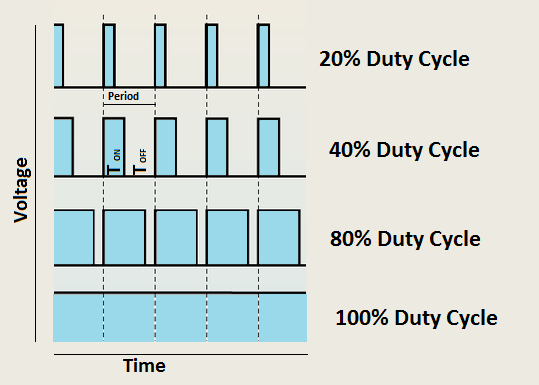
\includegraphics[keepaspectratio=true, width=0.95\textwidth]
            {img/pwm.png}
        \fonte{https://create.arduino.cc/projecthub/muhammad-aqib/arduino-pwm-tutorial-ae9d71}
        \label{fig:pwm}
    \end{minipage}
    \begin{minipage}{.5\textwidth}
        \centering
        \caption{Microcontrolador ESP32}
        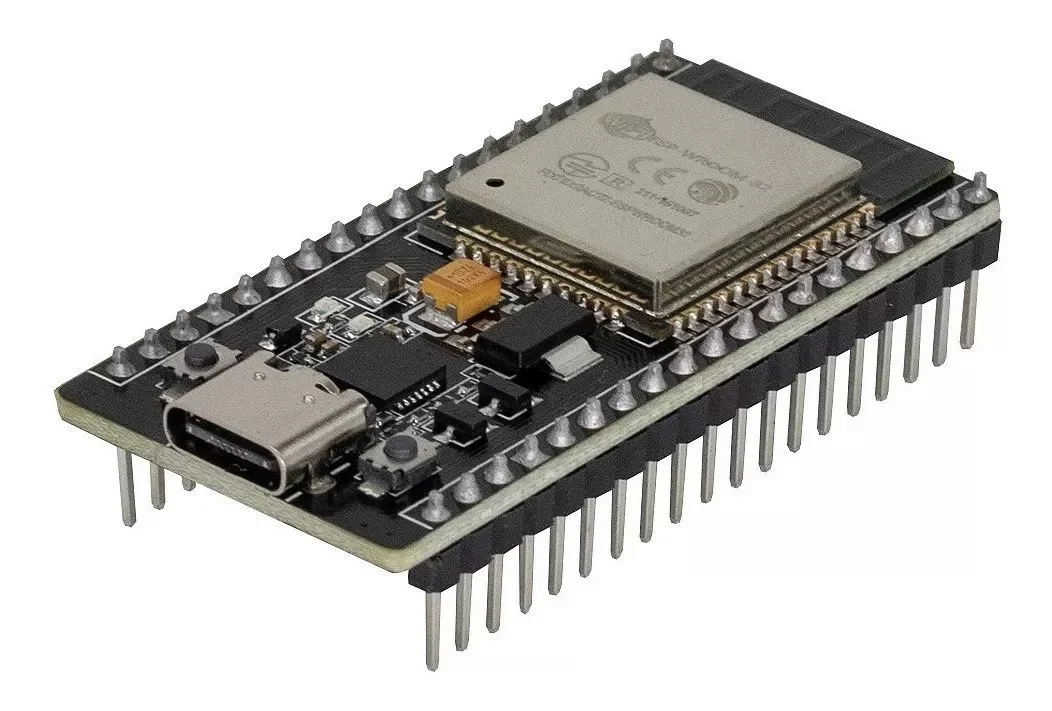
\includegraphics[keepaspectratio=true, width=0.95\textwidth]
            {img/foto-esp32.png}
        \fonte{https://www.robobuilders.com.br/nodemcu-esp32-38-pinos-devkit}
        \label{fig:fotoESP32}
    \end{minipage}%
\end{figure}

\subsection[Circuito de acionamento]{Circuito de acionamento}
\label{sub:circuitoAcionamento}

Para controlar os motores do manipulador, é necessário o uso de um circuito de acionamento para converter os sinais de baixa potência provenientes do microcontrolador em sinais de maior potência que movimentam as juntas do manipulador robótico.
Esse circuito é alimentado com 12 V, recebe sinais digitais de direção e de \textit{PWM} do ESP32 e envia sinais digitais para os motores do manipulador.

Para obter essa funcionalidade, foi decidido utilizar módulos de ponte H, que são circuitos integrados (CI) utilizados para aplicar uma tensão variável a um componente por meio de um sinal de \textit{PWM}.
Eles também permitem alterar a direção em que a corrente é aplicada no componente, o que possibilita inverter o sentido de rotação de um motor \cite{h_bridge}.
A Figura \ref{fig:ponteH} apresenta um módulo de ponte H disponível no mercado, que utiliza o CI L298N.

\begin{figure}[H]
    \centering
    \caption{Módulo de ponte H}
    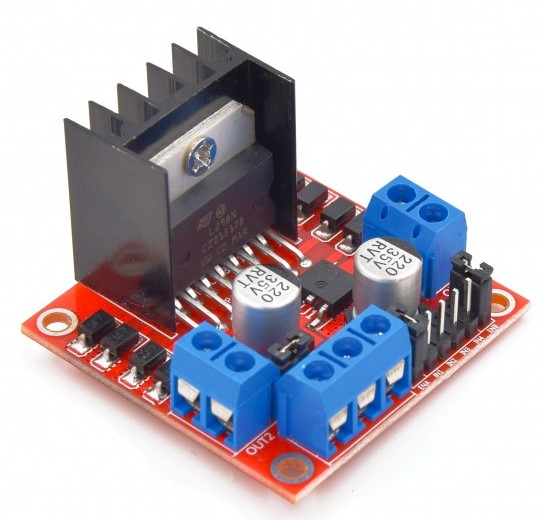
\includegraphics[keepaspectratio=true, width=0.5\textwidth]
    	{img/ponte-h.jpg}
    \fonte{https://www.smart-prototyping.com/L298N-Dual-H-bridge-Motor-Driver-Board}
    \label{fig:ponteH}
\end{figure}

\subsection[Computador]{Computador}
\label{sub:computador}

Para gerenciar o jogo de xadrez, foi decidido utilizar um computador.
Ele é responsável por implementar a lógica do jogo de xadrez e enviar sinais de controle para o ESP32, que por sua vez controla o manipulador robótico.

Para realizar a comunicação entre o computador e o ESP32, pode ser usado o protocolo serial, através de um cabo USB.
Através dele o computador envia sinais indicando para qual casa do tabuleiro o manipulador deve mover, e quando ele deve pegar ou soltar uma peça.
Por outro lado, o ESP32 envia sinais indicando quando o movimento foi finalizado e, no modo manual, qual movimento o jogador deseja realizar.

Para implementar as regras do jogo, é necessário desenvolver um \textit{software} para interagir com uma \textit{engine} de xadrez.
Essa \textit{engine} é um \textit{software} que implementa as regras do jogo e permite que o computador jogue xadrez contra um humano ou contra outro computador.
Ao integrar o \textit{software} desenvolvido com uma \textit{engine}, é possível verificar quais movimentos são válidos, determinar qual movimento será jogado pelo computador e identificar quando o jogo terminou.
Por fim, o computador também é responsável por converter um movimento em uma sequência de comandos que devem ser enviados ao ESP32.

\section[Projeto do sistema]{Projeto do sistema}
\label{sec:projetoSistema}

Após a definição de todos os equipamentos a serem utilizados, foi feito o projeto do sistema,
indicando como os componentes devem ser conectados.

A manete deve ser alimentada com 3,3 V e ser conectada ao ESP32 para permitir a leitura dos sinais de entrada.
Essa conexão é realizada com 10 cabos, sendo 5 para cada \textit{joystick} com seu respectivo botão.

O circuito de acionamento deve ser alimentado com 12 V e também deve ser conectado ao ESP32 para receber os sinais de controle.
Essa conexão é realizada com 10 cabos, 2 para o controle de cada junta do manipulador robótico.
Essa circuito também deve ser conectado aos motores do manipulador robótico, também com 10 cabos, 2 para cada junta.

O manipulador robótico deve ser conectado ao ESP32 para o envio dos sinais de posição de cada junta.
Essa conexão é realizada com 5 cabos, um para cada junta.

Por fim, o ESP32 deve ser alimentado com 3,3 V e deve ser conectado a um computador para a implementação da lógica do jogo.

A montagem do sistema é mostrada na Figura \ref{fig:montagemSistema}.

\begin{figure}[H]
    \centering
    \caption{Montagem do sistema}
    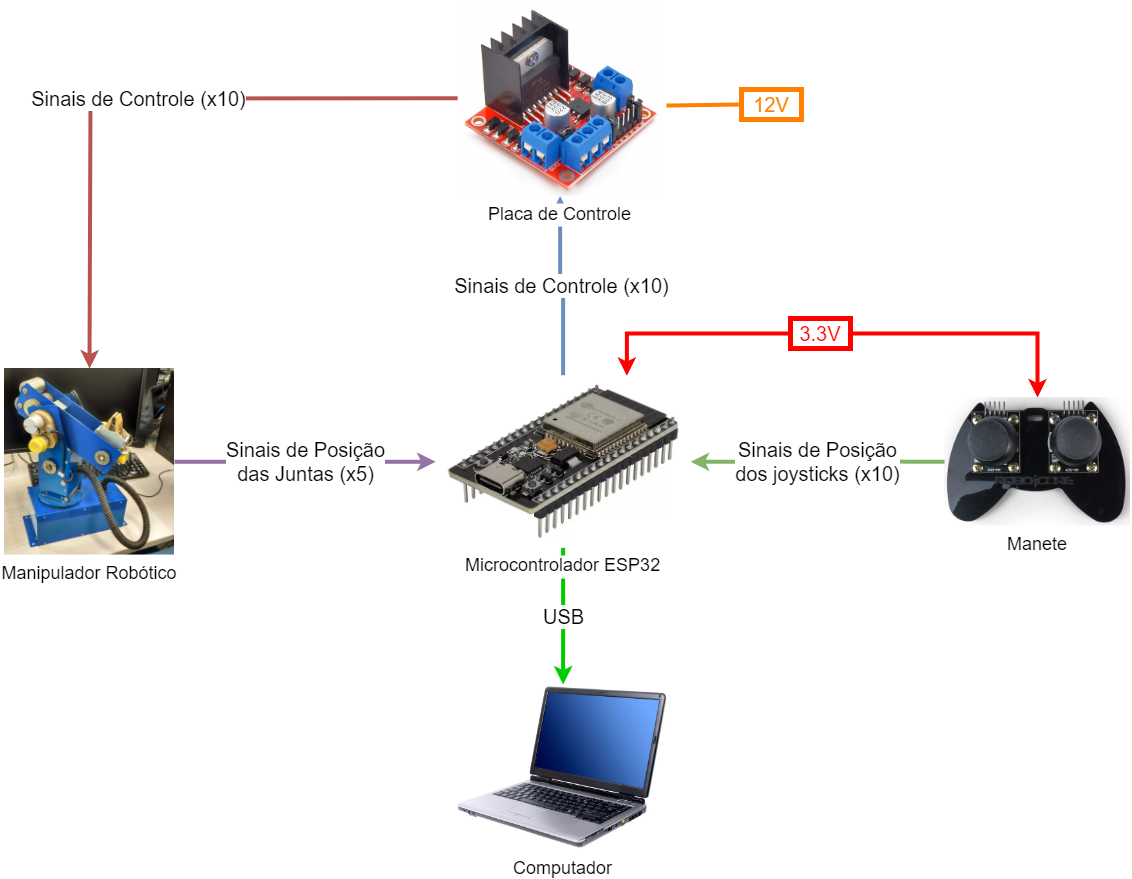
\includegraphics[keepaspectratio=true, width=0.8\textwidth]
    	{img/projeto-sistema.png}
    \fonte{Do próprio autor}
    \label{fig:montagemSistema}
\end{figure}


